\documentclass[8pt]{beamer}

\usetheme{UM}
\usecolortheme{UM}
% \setbeamertemplate{page number in head/foot}[totalframenumber]

\usepackage{datetime}
\usepackage{amsmath, amsthm, amsfonts, amssymb}
% \usepackage{mathtools}
\usepackage{float}
\usepackage{enumerate}
\usepackage{graphicx}
\usepackage{overpic}
\usepackage{tikz}
\usepackage{tikz-cd}

% \newtheorem{theorem}{Theorem}[section]
% \newtheorem*{untheorem}{Theorem}

% \newtheorem{lemma}[theorem]{Lemma}

% \newtheorem{claim}[theorem]{Claim}
\newtheorem{proposition}[theorem]{Proposition}
% \newtheorem{corollary}[theorem]{Corollary}
\newtheorem{conjecture}[theorem]{Conjecture}
\newtheorem{goal}[theorem]{Goal}

% \theoremstyle{definition}
% \newtheorem{example}[theorem]{Example}
% \newtheorem*{fact}{Fact}

% \theoremstyle{definition}
% \newtheorem{question}[theorem]{Question}
% \newtheorem*{unquestion}{Question}

% \theoremstyle{remark}
% \newtheorem*{remark}{Remark}
% \newtheorem*{proofsketch}{Outline of proof}

% \theoremstyle{definition}
% \newtheorem{definition}[theorem]{Definition}

\newcommand{\pmf}{\mathbb{P}\mathcal{MF}}
\newcommand{\mf}{\mathcal{MF}}
\newcommand{\mcg}{\text{MCG}}
\newcommand{\os}{\mathcal{S}}
\newcommand{\no}{\mathcal{N}}
\newcommand{\teich}{\mathrm{Teich}}
\newcommand{\mg}{\mathcal{M}}
\newcommand{\pslr}{\text{PSL}(2, \mathbb{R})}
\newcommand{\scc}{\mathscr{S}}
\newcommand{\QQ}{\mathbb{Q}}
\newcommand{\ZZ}{\mathbb{Z}}
\newcommand{\wt}{\widetilde}
\newcommand{\cA}{\mathcal{A}}
\newcommand{\cR}{\mathcal{R}}
\newcommand{\dynlim}{\Lambda_{\text{dyn}}}
\newcommand{\geolim}{\Lambda_{\text{geo}}}
\newcommand{\HH}{\mathbb{H}^2}
\newcommand{\RR}{\mathbb{R}}
\newcommand{\expansion}{\text{Sat}}
\newcommand{\err}[1]{\text{err}_{#1}}
\newcommand{\norm}[1]{\left\lVert#1\right\rVert}
\newcommand{\dd}{\text{\,d}}
\newcommand{\lhyp}{\ell_{\text{hyp}}}
\newcommand{\lflat}{\ell_{\text{flat}}}
\renewcommand{\qedsymbol}{}


\newcommand\Narrower[2][3em]{%
\makebox[\linewidth][c]{%
  \begin{minipage}{\dimexpr\textwidth-#1\relax}
  \raggedright#2
  \end{minipage}%
  }%
}

\def\signed #1{{\leavevmode\unskip\nobreak\hfil\penalty50\hskip2em
  \hbox{}\nobreak\hfil(#1)%
  \parfillskip=0pt \finalhyphendemerits=0 \endgraf}}

\newsavebox\mybox
\newenvironment{aquote}[1]
  {\savebox\mybox{#1}\begin{quote}}
  {\signed{\usebox\mybox}\end{quote}}


\setbeamercolor{block title}{fg=black, bg=pink}

\title{Dynamics on the Moduli Space of Non-Orientable Surfaces}
\author[Sayantan Khan]{Sayantan Khan}
\institute{University of Michigan}

% \newdate{date}{2}{4}{2024}
\date{Tuesday, April 2\textsuperscript{nd} 2024}

\subject{Mathematics}

% \setbeamertemplate{footline}[page number]{}

% Delete this, if you do not want the table of contents to pop up at
% the beginning of each subsection:
% \AtBeginSection[]
% {
%   \begin{frame}<beamer>{Outline}
%     \tableofcontents[currentsection]
%   \end{frame}
% }


\begin{document}

\begin{frame}
  \titlepage
\end{frame}

\section{Moduli spaces of non-orientable surfaces}

\begin{frame}
\begin{columns}
\begin{column}{0.5\textwidth}
  \begin{center}
    Orientable surfaces \\
    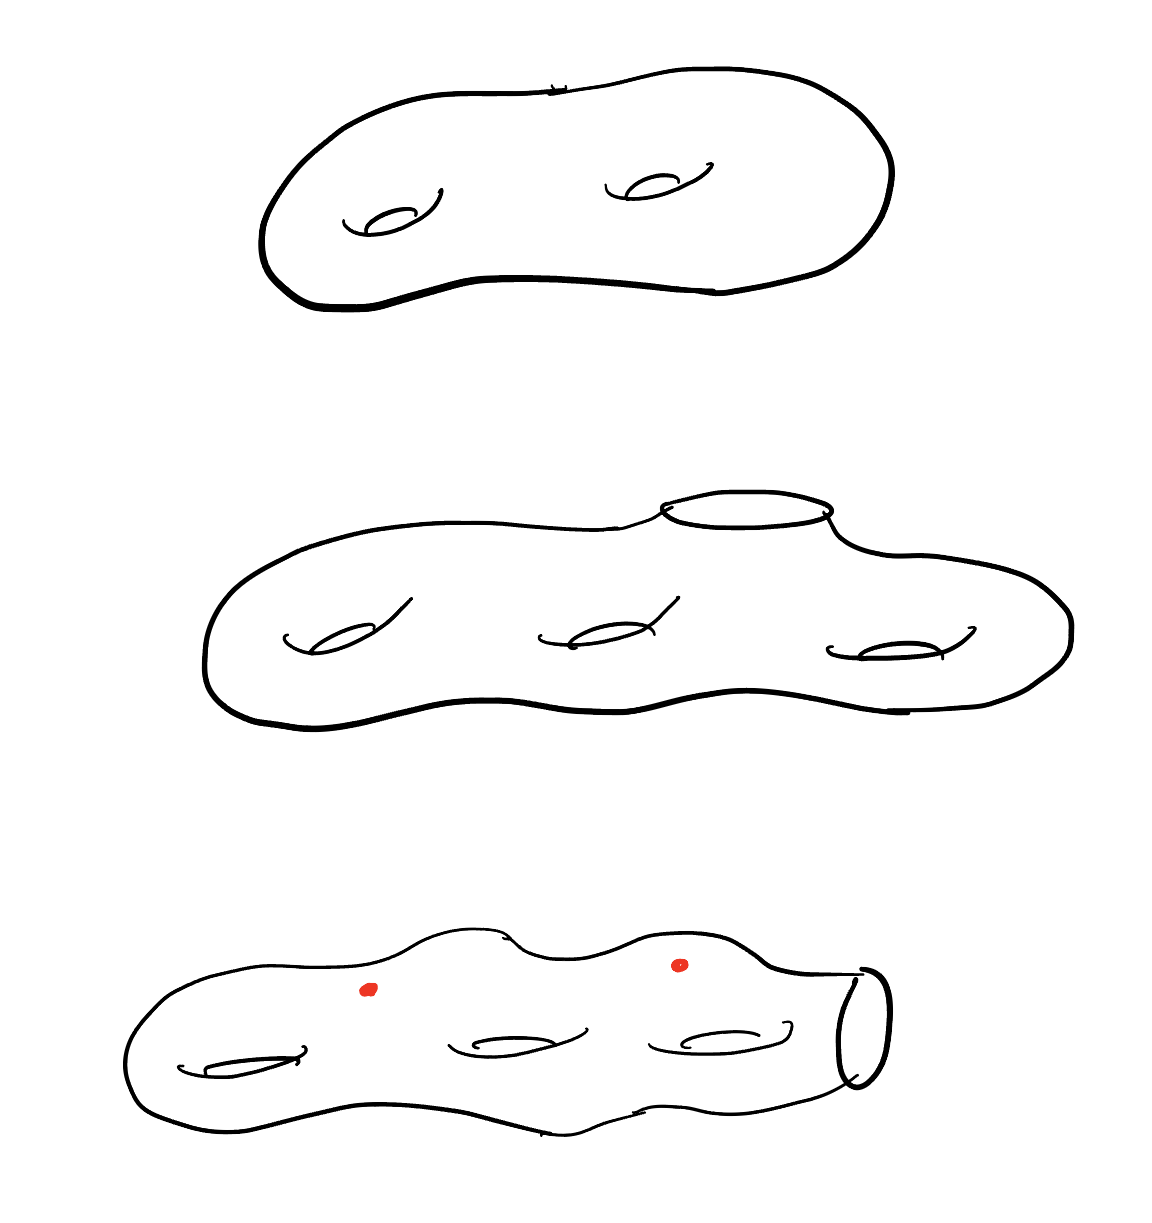
\includegraphics[scale=0.15]{orientable.png}
  \end{center}
\end{column}
\pause
\begin{column}{0.5\textwidth}  %%<--- here
    \begin{center}
      Non-orientable surfaces
      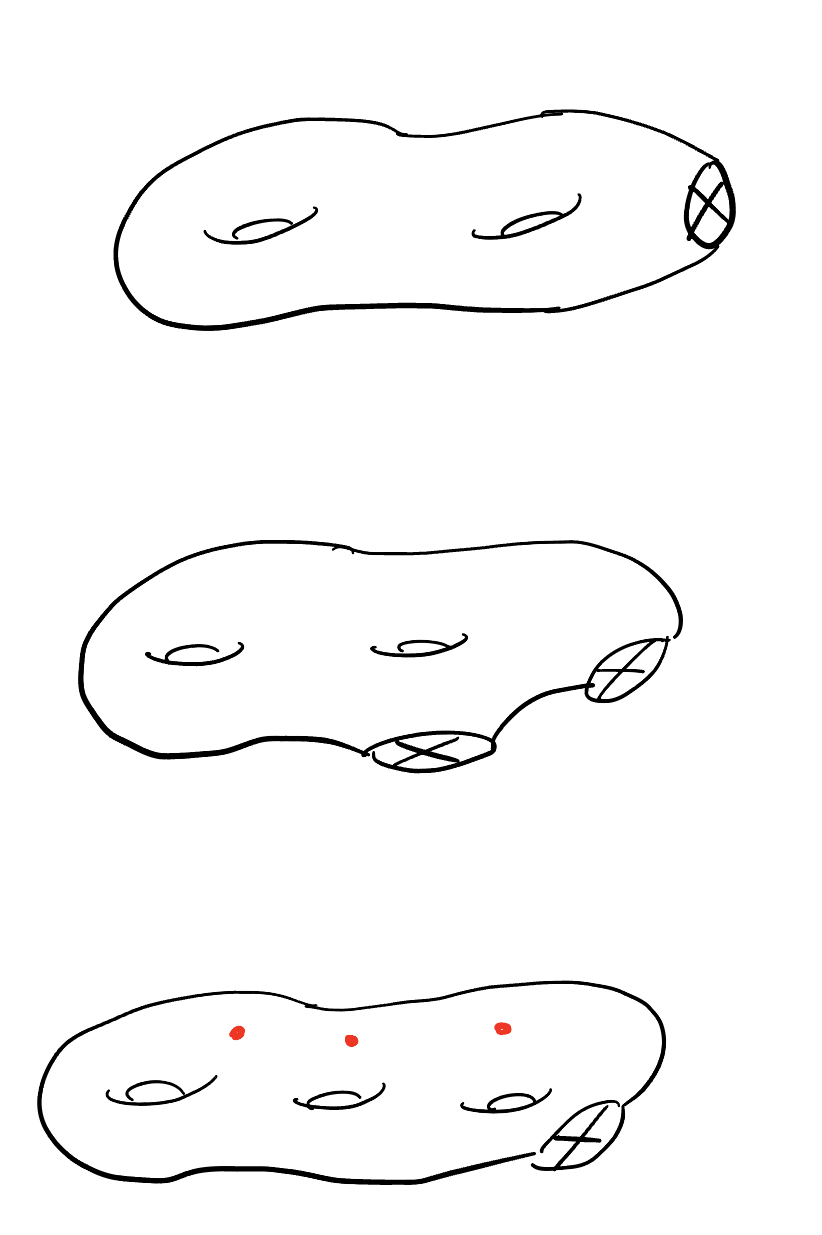
\includegraphics[scale=0.15]{nonorientable.png}
     \end{center}
\end{column}
\end{columns}
\end{frame}

\begin{frame}
  \begin{goal}
    Understand the collection of geometric structures we can put on a topological surface.
  \end{goal}
  \pause
  In particular, understand the set of metrics on a surface with curvature $-1$.
  \begin{figure}[h]
    \centering
    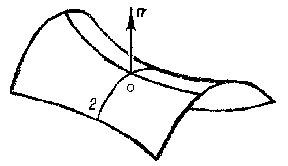
\includegraphics[scale=0.5]{negative-curvature.png}
  \end{figure}
\end{frame}

\begin{frame}
  \begin{align*}
    \mg(\os_g) = \left\{ \text{Curvature $-1$ metrics on $\os_g$} \right\}
  \end{align*}
  \begin{itemize}
  \item<2-> $\mg(\os_g)$ is $6g-6$ dimensional.
  \item<3-> $\mg(\os_g)$ is a metric space: $x$ and $y$ in $\mg(\no_g)$ are close if the derivative of some map $x \to y$ maps circles to ``almost'' circles.
  \item<4-> Unit (co)tangent bundle of $\mg(\os_g)$ is non-compact, but finite volume, and admits a geodesic flow (and an $SL(2, \mathbb{R})$ action) with good dynamical properties.
  \end{itemize}
  \uncover<5->{
  \textbf{Guiding principle}: Dynamics on (co)tangent bundle should have analogies with dynamics of the $SL(2, \mathbb{R})$ action on $SL(2, \mathbb{R})/SL(2, \mathbb{Z})$.
  }
\end{frame}

\begin{frame}
  \begin{align*}
    S^1 \mg(\os_g) = \left\{ \text{Area $1$ half-translation surface structures on $\os_g$} \right\}
  \end{align*}
  \uncover<2->{
    \begin{figure}[h]
      \centering
      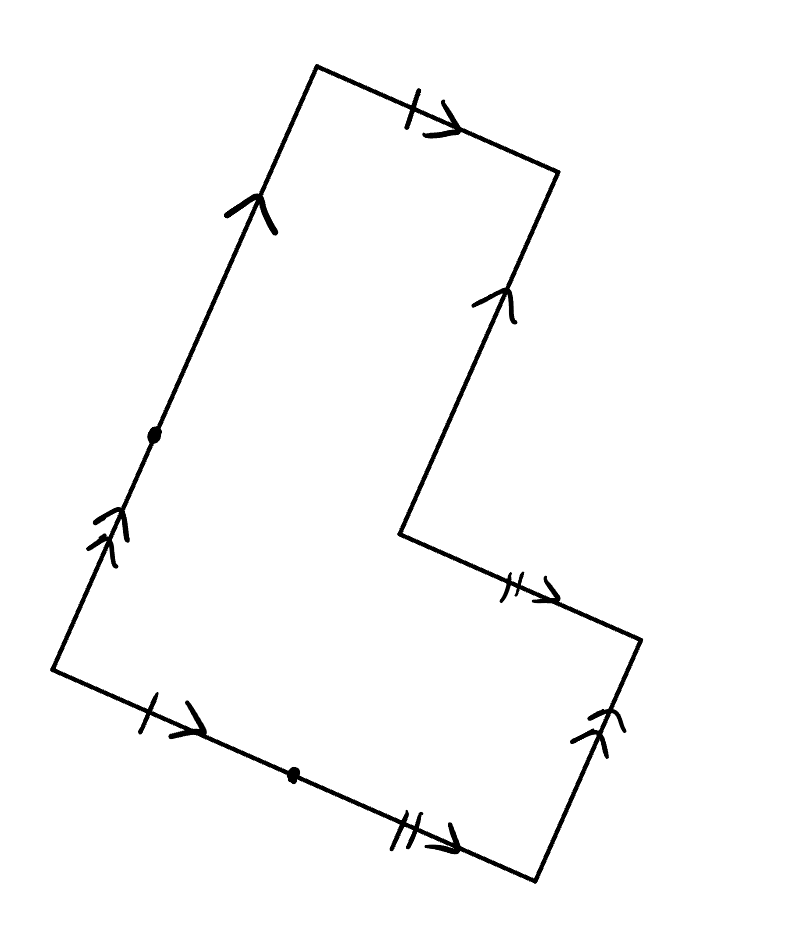
\includegraphics[scale=0.1]{tangent.png}
    \end{figure}
  }

  \uncover<3->{
    \begin{theorem}[Masur's criterion]
      If the vertical flow on translation surface is not uniquely ergodic, then the geodesic ray in $\mg(\os_g)$ escapes to infinity.
    \end{theorem}
  }
\end{frame}

\begin{frame}
  \begin{align*}
    \mg(\no_g) = \left\{ \text{Curvature $-1$ metrics on $\no_g$} \right\}
  \end{align*}
  \begin{itemize}
  \item<2-> $\mg(\no_g)$ is $3g-6$ dimensional.
  \item<3-> $\mg(\no_g)$ is a metric space, with a similarly defined metric.
  \item<4-> Unit (co)tangent bundle of $\mg(\no_g)$ is non-compact, and also infinite volume (with respect to the canonical volume form).
  \item<5->  $S^1 \mg(\no_g)$ admits a geodesic flow but not an $SL(2, \mathbb{R})$ action: however, the dynamical properties are not great.
  \end{itemize}
  \uncover<6->{
  \textbf{Guiding principle?}
  }
\end{frame}

\begin{frame}
  \begin{goal}
    Analyze generic tangent vector in $S^1 \mg(\no_g)$.
  \end{goal}
  \begin{itemize}
  \item<2-> Analyze vertical flow on translation surface.
  \item<3-> Will suffice to look at first return map to a horizontal arc.
  \end{itemize}
    \begin{figure}[h]
      \begin{overprint}
      \centering
      \onslide<4>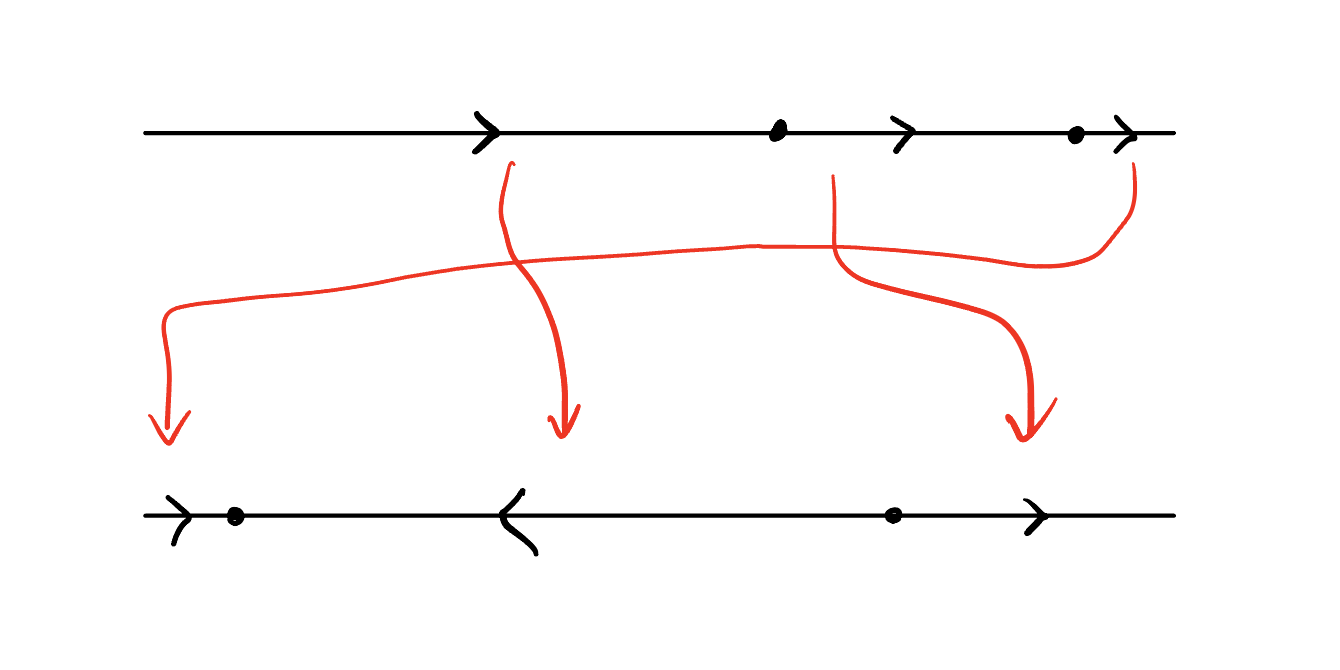
\includegraphics[scale=0.2]{ietwf.png}
      \onslide<5->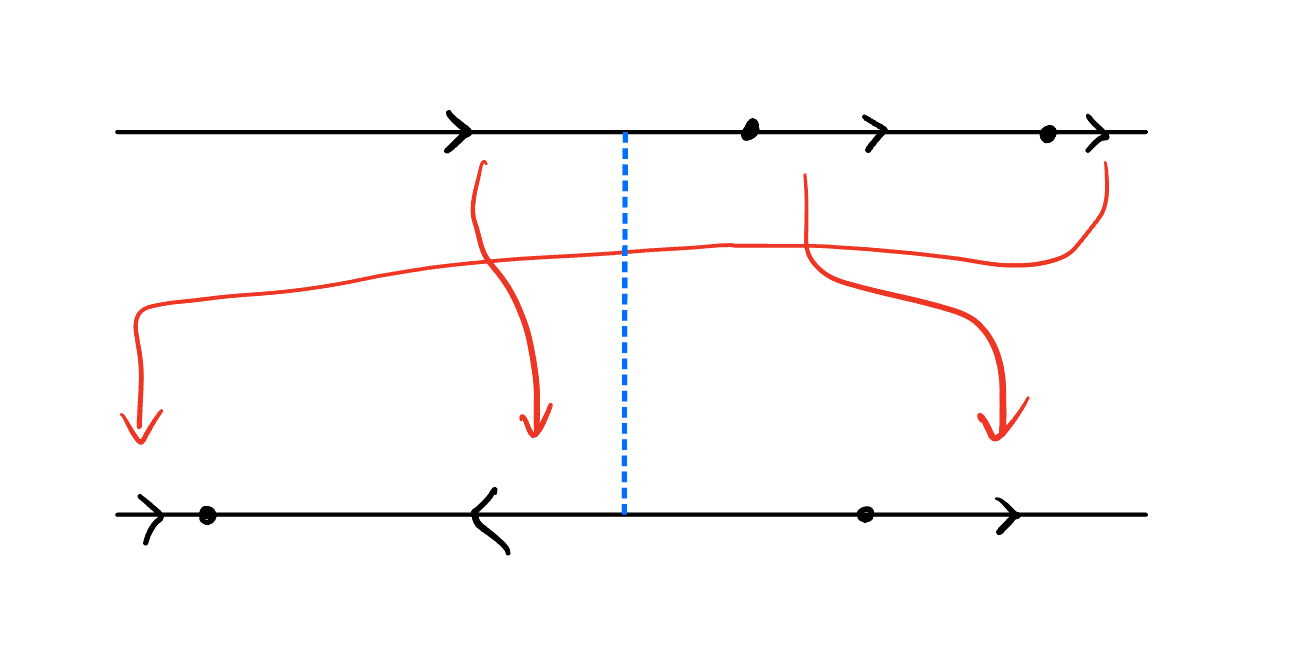
\includegraphics[scale=0.2]{ietwf2.png}
      \end{overprint}
    \end{figure}
    \uncover<6->{
      \begin{theorem}
        Almost every geodesic in $S^1\mg(\no_g)$ escapes to infinity.
      \end{theorem}
    }

\end{frame}

\begin{frame}
 \begin{columns}
\begin{column}{0.5\textwidth}
  \begin{center}
    $\mcg(\no_g)$-action on $\teich(\no_g)$ \\
  \end{center}
  \begin{itemize}
  \item<2-> $\mcg(\no_g)$ is finitely generated.
  \item<3-> The action is infinite covolume.
  \item<4-> Almost no geodesics recur.
  \item<10-> \textbf{Question}: What is the limit set for the $\mcg(\no_g)$ action?
  \item<12-> \textbf{Question}: Can we construct a Patterson-Sullivan measure on the limit set with ``good'' dynamical properties?
  \end{itemize}
\end{column}
\uncover<5-> {
\begin{column}{0.5\textwidth}  %%<--- here
    \begin{center}
      Geometrically finite $\Gamma$ action on $\mathbb{H}$
     \end{center}
     \begin{itemize}
     \item<6-> $\Gamma$ is finitely generated.
     \item<7-> $\Gamma$ action is infinite covolume (with respect to the Liouville measure).
     \item<8-> Almost no geodesics recur.
     \item<9-> Limit set of $\Gamma$ is a subset of the boundary with smaller Hausdorff dimension.
     \item<11-> Have a Patterson-Sullivan measure on the limit set with ``good'' dynamical properties.
     \end{itemize}
\end{column}
}

\end{columns}
\uncover<13->{
  \begin{theorem}[K., Erlandsson-Gendulphe-Pasquinelli-Souto]
    The limit set of the $\mcg(\no_g)$ action on $\teich(\no_g)$ is $\pmf^+(\no_g)$.
  \end{theorem}
}
\end{frame}

\end{document}
